\section{Esempi d'uso}
Una volta raggiunta la pagina iniziale dell'applicazione l'utente deve registrarsi o effettuare il Login qualora avesse già un account.

\begin{figure}[H]
    \caption{Schermata di Login (Finale)}
    \centering
    \fbox{
    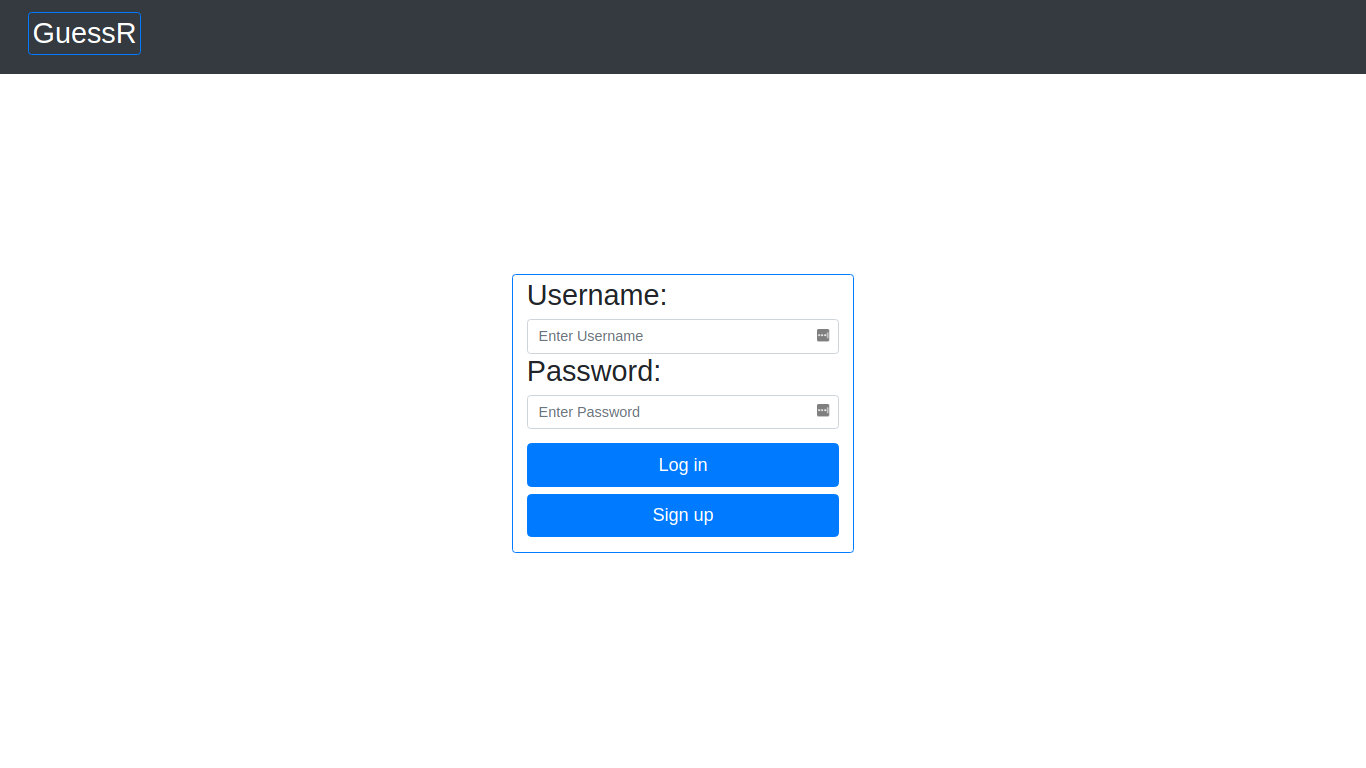
\includegraphics[width=135mm]{img/screen/login_screen.png}
    }
    \label{fig:login_screen}
\end{figure}

\noindent Una volta effettuato l'accesso l'utente si troverà davanti al menù principale. Sarà possibile creare una nuova Lobby o accedere ad una già esistente. Per creare una Lobby è necessario cliccare il pulsante \textit{``Create Lobby"}.

\begin{figure}[H]
    \caption{Schermata del Menù Principale (Finale)}
    \centering
    \fbox{
    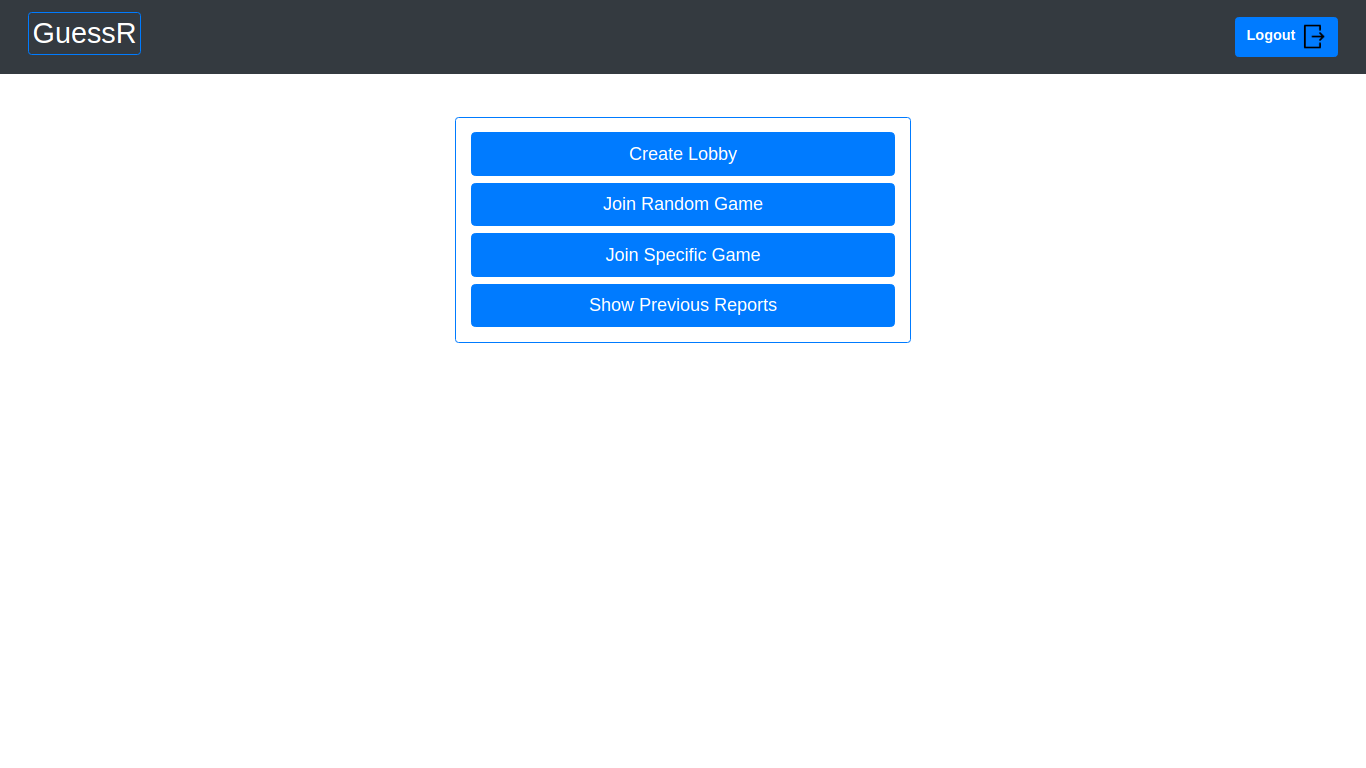
\includegraphics[width=135mm]{img/screen/main_menu_screen.png}
    }
    \label{fig:menu_screen}
\end{figure}

\noindent Nella schermata di creazione della Lobby è possibile impostare alcuni parametri: la visibilità della lobby, il numero di turni da giocare, la lingua in cui giocare.\newline
Una volta finita la configurazione è possibile creare una lobby.

\begin{figure}[H]
    \caption{Schermata della creazione della Lobby (Finale)}
    \centering
    \fbox{
    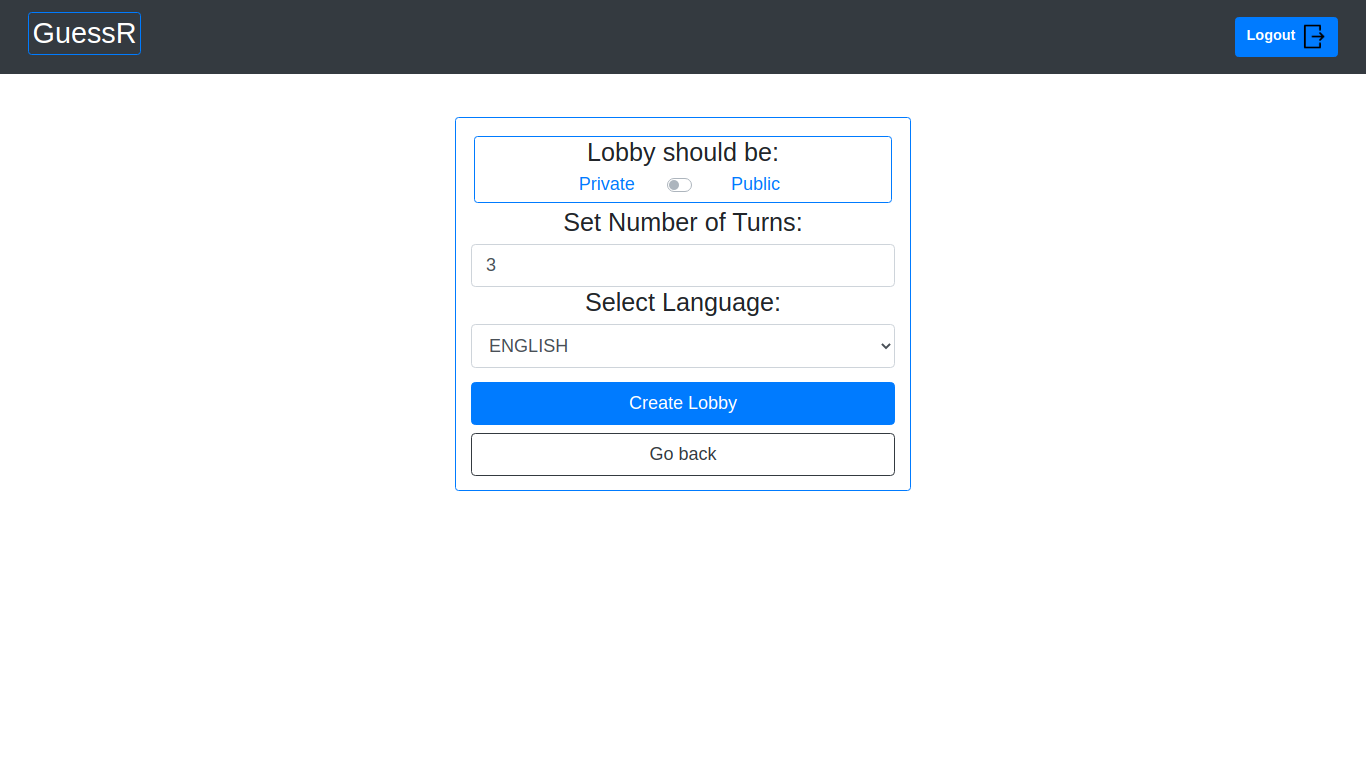
\includegraphics[width=135mm]{img/screen/lobby_creation.png}
    }
    \label{fig:lobby_create_screen}
\end{figure}

\noindent Una volta creata, sarà possibile per altri utenti entrare. Se la lobby è privata solo i giocatori in possesso del codice potranno entrare. Se la lobby è pubblica chiunque può entrare e giocare. Una volta che ci saranno almeno tre giocatori, l'utente che ha creato la lobby potrà iniziare la partita.
\begin{figure}[H]
    \caption{Schermata dell'attesa in Lobby (Finale)}
    \centering
    \fbox{
    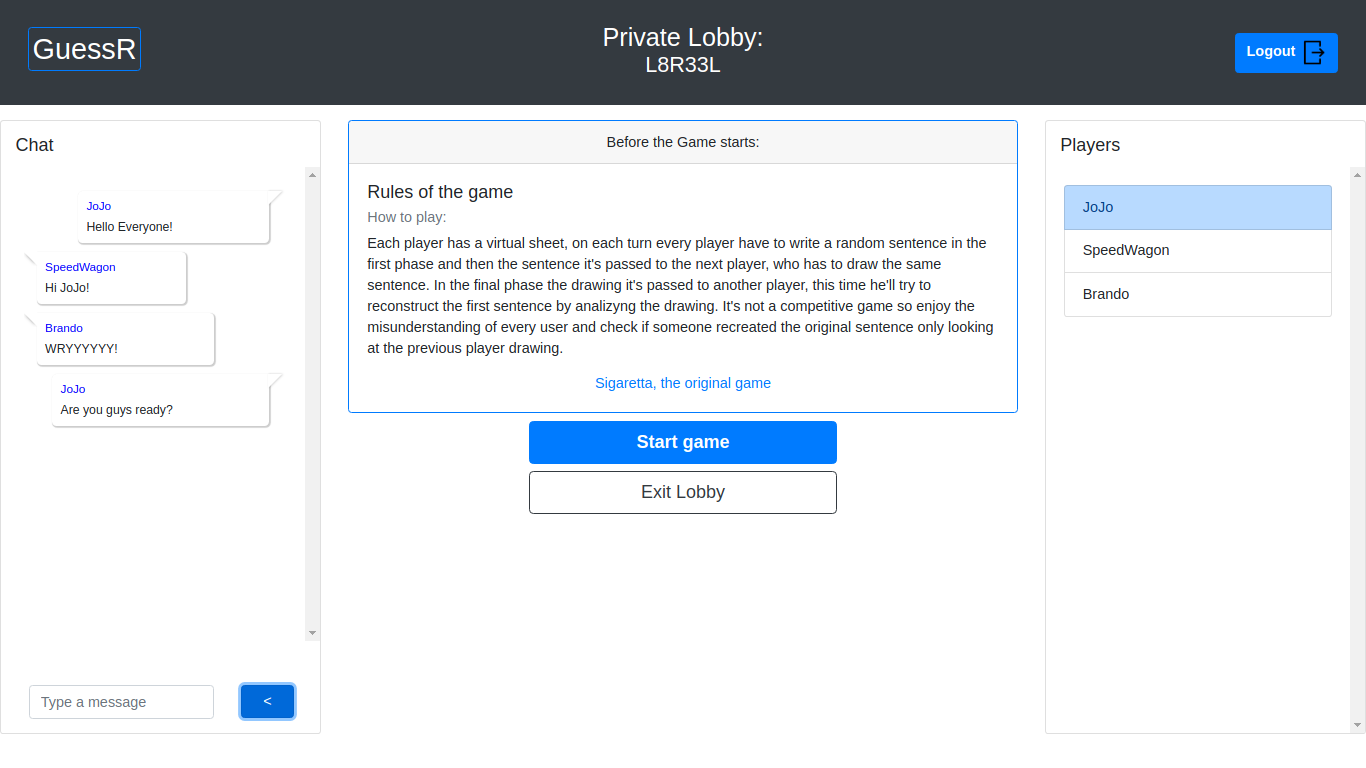
\includegraphics[width=135mm]{img/screen/inside_lobby_screen.png}
    }
    \label{fig:in_lobby_screen}
\end{figure}

\noindent La prima cosa che viene richiesta ad ogni giocatore è la scrittura di una frase inventata sul momento. Una volta decisa, l'utente dovrà inserirla nel box di testo a sua disposizione e premere sul tasto \textit{``Submit"}. Il tempo a disposizione per scrivere la frase è un minuto.
\begin{figure}[H]
    \caption{Schermata di gioco, fase di scrittura della frase (Finale)}
    \centering
    \fbox{
    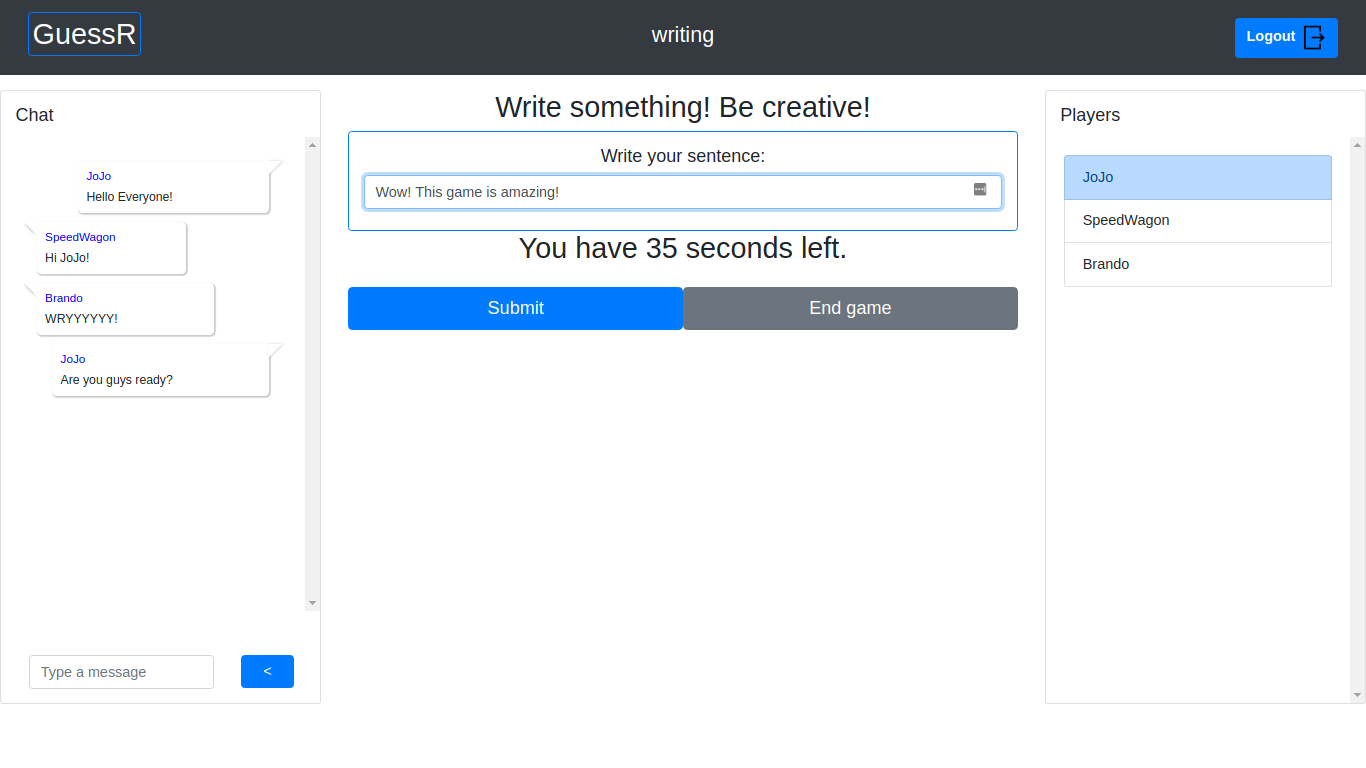
\includegraphics[width=135mm]{img/screen/sentence_screen.png}
    }
    \label{fig:sentence_screen}
\end{figure}

\noindent Una volta che tutti gli utenti in partita avranno inviato la loro frase si passerà alla fase successiva. Gli utenti dovranno disegnare nel box messo a disposizione la frase che vedono a schermo. Il tempo a disposizione per disegnare è di due minuti. Una volta che tutti gli utenti avranno inviato il proprio disegno si ritornerà alla fase in cui va inserita una frase. Questa volta sarà necessario descrivere a parole in disegno sullo schermo. Questo ciclo \textit{frase-disegno} andrà avanti fino a quando non saranno finiti i turni impostati dal creatore della lobby.

\begin{figure}[H]
    \caption{Schermata di gioco, fase di disegno (Finale)}
    \centering
    \fbox{
    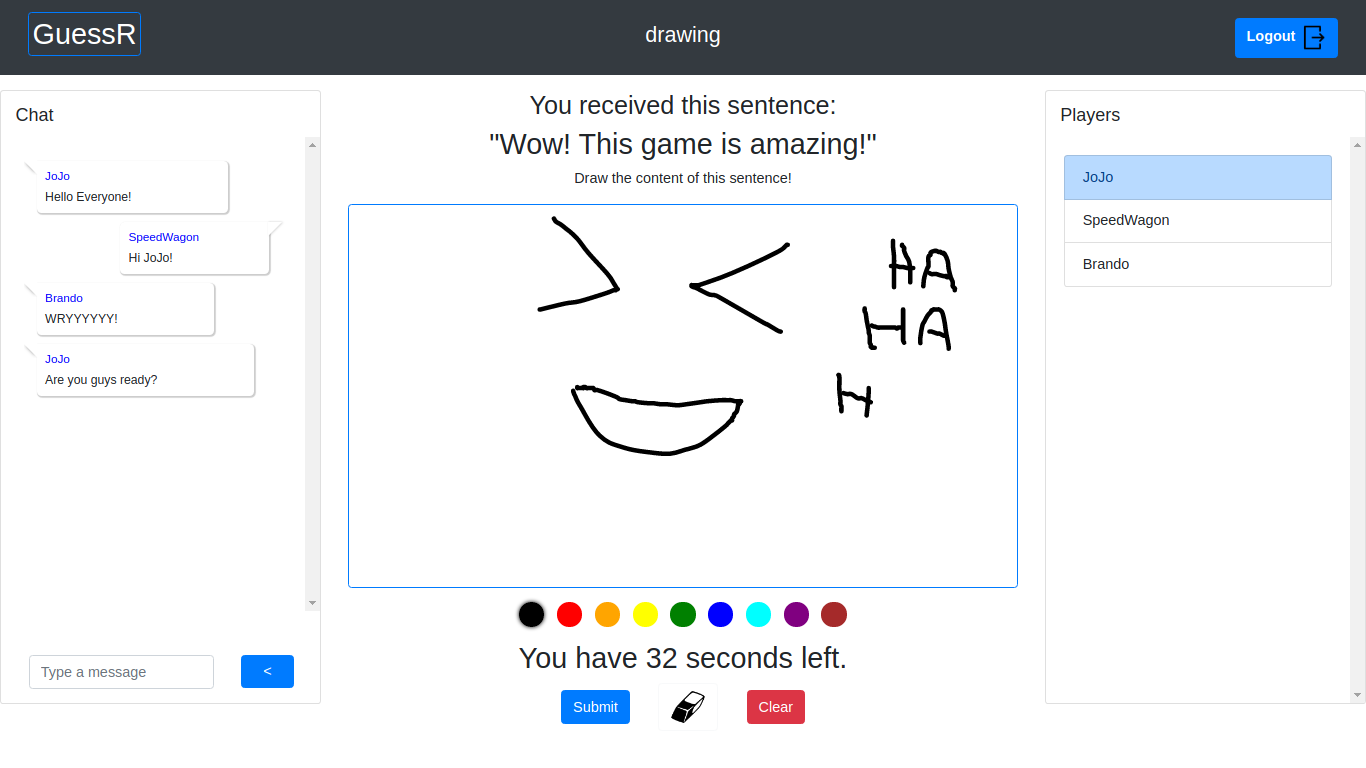
\includegraphics[width=135mm]{img/screen/drawing_phase.png}
    }
    \label{fig:draw_screen}
\end{figure}
 \noindent Una volta che i turni saranno finiti, tutti gli utenti verranno reindirizzati alla pagina in cui vengono visualizzati i risultati finali. Compariranno tanti bottoni quanti sono i giocatori, ognuno rappresentante il foglio in cui quel giocatore ha scritto per primo.

\begin{figure}[H]
    \caption{Schermata di fine gioco, report chiusi (Finale)}
    \centering
    \fbox{
    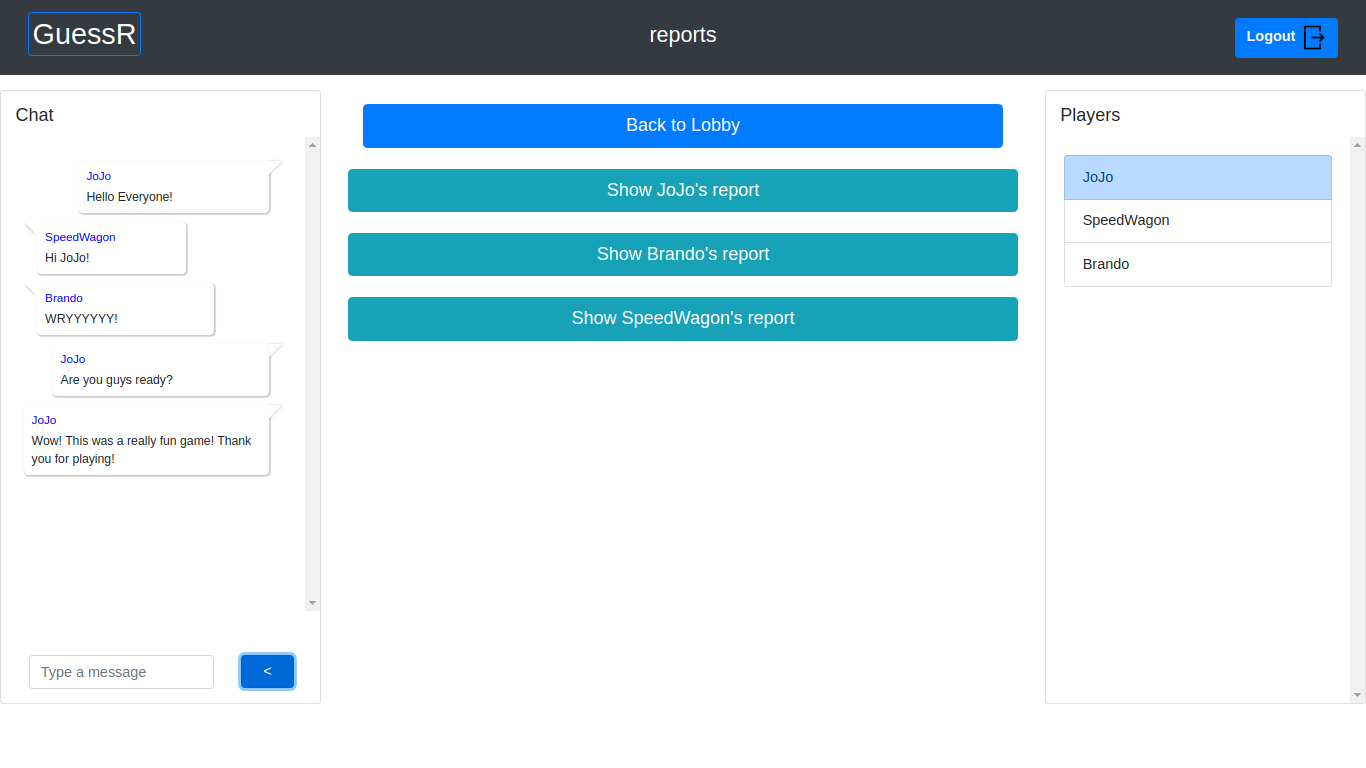
\includegraphics[width=135mm]{img/screen/end_game_screen.png}
    }
    \label{fig:end_game}
\end{figure}

\noindent Cliccando su un bottone verrà mostrato l'intero foglio. A questo punto il creatore della Lobby può scegliere se iniziare una nuova partita o andarsene.

\begin{figure}[H]
    \caption{Schermata di fine gioco, primo report aperto (Finale)}
    \centering
    \fbox{
    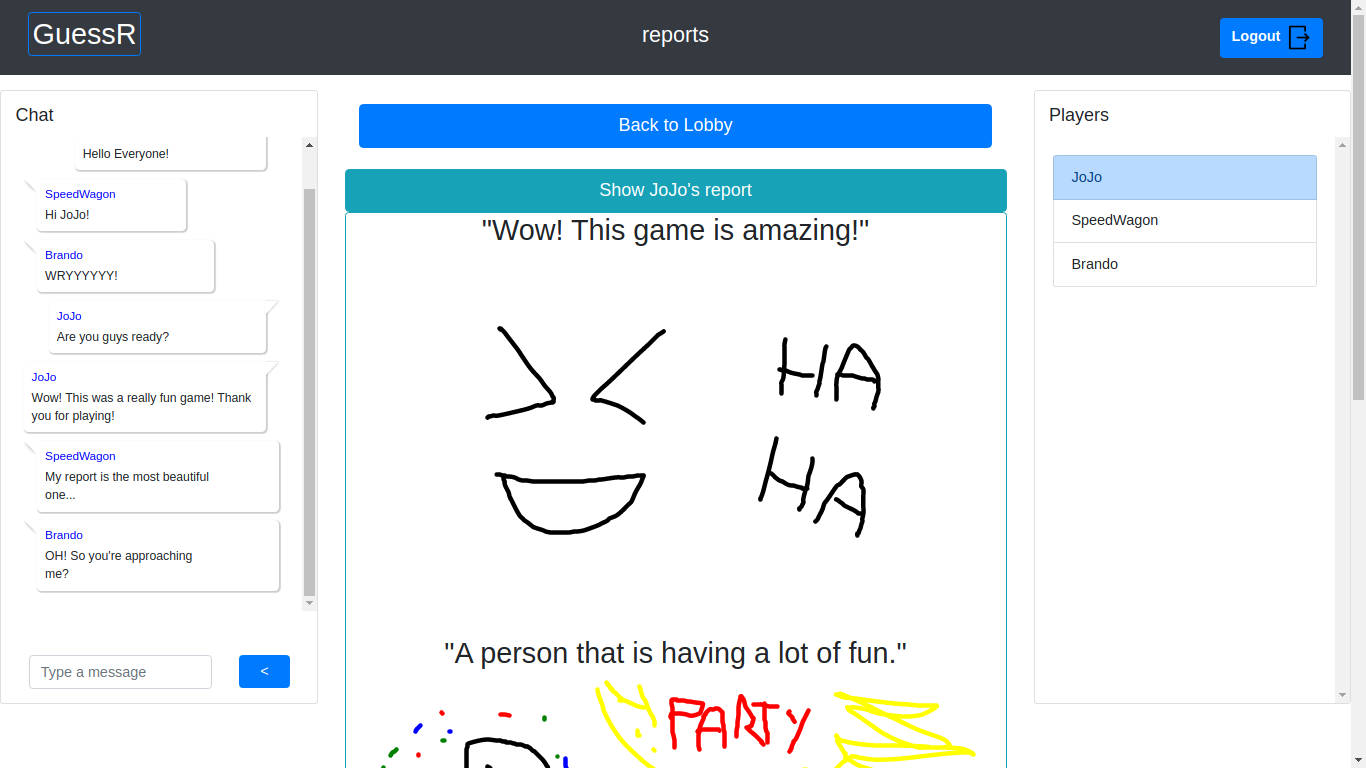
\includegraphics[width=135mm]{img/screen/end_game_2_screen.png}
    }
    \label{fig:end_game_2}
\end{figure}

\noindent Se un utente si è particolarmente divertito durante una partita potrebbe voler conservare un record come ricordo.
Dal Menù principale è possibile cliccare sul tasto \textit{``Show Previous Reports"} per visualizzare tutti i report passati. Cliccando sul pulsante ``Download PDF" sarà possibile scaricare un file in locale contenente le frasi e disegni quel report.
\begin{figure}[H]
    \caption{Schermata dei report passati (Finale)}
    \centering
    \fbox{
    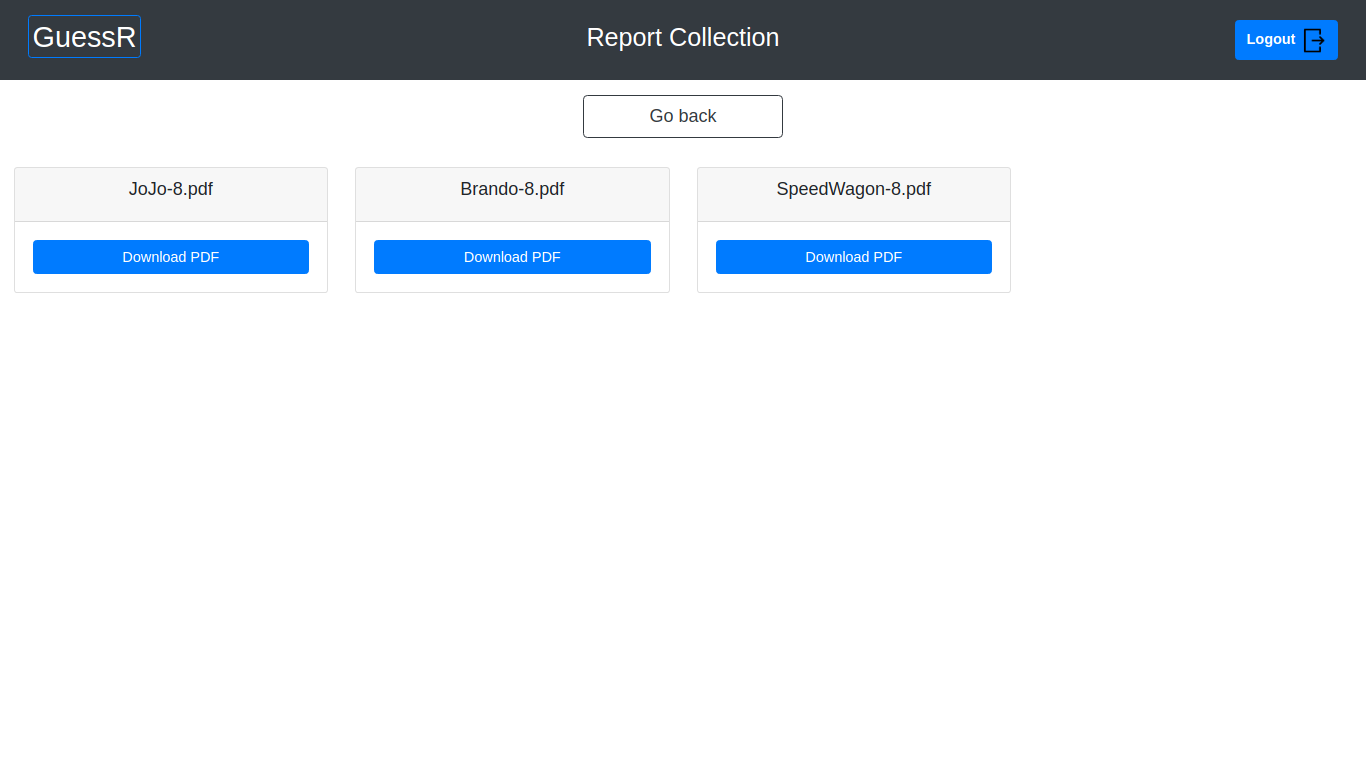
\includegraphics[width=135mm]{img/screen/previous_report_screen.png}
    }
    \label{fig:previous_report}
\end{figure}

\newpage
